\documentclass[tikz,convert={outfile=fonctions.png}]{standalone}

    \usepackage[utf8]{inputenc}

\begin{document}
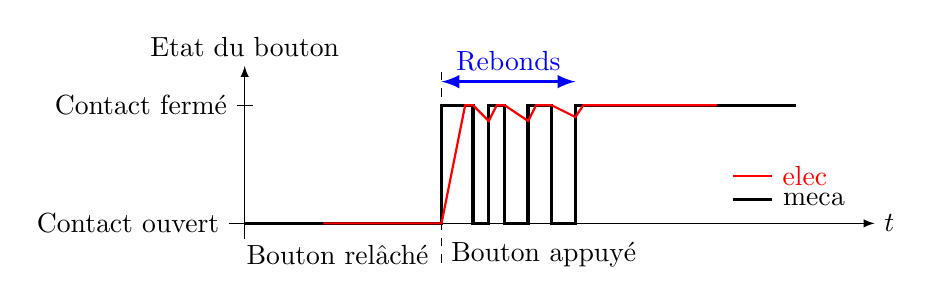
\begin{tikzpicture}[>=latex]

    \draw[->] (-.2,0) -- (8,0) node[right] {$t$};
    \draw[->] (0,-.2) -- (0,2) node[above] {Etat du bouton};

    \draw (-.2,0) node[left] {Contact ouvert};
    \draw (.1,1.5) -- ++(-.2,0) node[left] {Contact fermé};

    % point de contact
    \draw[dashed] (2.5,-.5) -- ++(0,2.5);
    \draw (-.1,-.4) node[right] {Bouton relâché};
    \draw (2.5,-.4) node[right] {Bouton appuyé};
    \draw[<->, very thick, blue] (2.5,1.8) -- (4.2,1.8) node[midway, above, blue] {Rebonds};

    % signal meca
    \draw[very thick] (0,0) -- (2.5,0) -- (2.5,1.5)
        % rebonds
        -- ++(.4,0) -- ++(0,-1.5) -- ++(.2,0) -- ++(0,1.5)
        -- ++(.2,0) -- ++(0,-1.5) -- ++(.3,0) -- ++(0,1.5)
        -- ++(.3,0) -- ++(0,-1.5) -- ++(.3,0) -- ++(0,1.5)
        % fin de signal
        -- (7,1.5);

    % signal elec
    \draw[thick, red] (1,0) -- (2.5,0) -- (2.8,1.5)
        % rebonds
        -- ++(.1,0) -- ++(.2,-.2)
        -- ++(.1,.2) -- ++(.1,0) -- ++(.3,-.2)
        -- ++(.1,.2) -- ++(.2,0) -- ++(.3,-.15) -- ++(.1,.15)
        % fin de signal
        -- (6,1.5);

    \draw[very thick] (6.2,0.3) -- ++(.5,0) node[right] {meca};
    \draw[thick, red] (6.2,0.6) -- ++(.5,0) node[right] {elec};
   
\end{tikzpicture}
\end{document}

